%% bare_conf.tex V1.2
%% 2002/11/18
%% by Michael Shell
%% mshell@ece.gatech.edu
%% 
%% This is a skeleton file demonstrating the use of IEEEtran.cls 
%% (requires IEEEtran.cls version 1.6b or later) with an IEEE conference paper.
%% 
%% Support sites:
%% http://www.ieee.org
%% and/or
%% http://www.ctan.org/tex-archive/macros/latex/contrib/supported/IEEEtran/ 
%%
%% This code is offered as-is - no warranty - user assumes all risk.
%% Free to use, distribute and modify.

% *** Authors should verify (and, if needed, correct) their LaTeX system  ***
% *** with the testflow diagnostic prior to trusting their LaTeX platform ***
% *** with production work. IEEE's font choices can trigger bugs that do  ***
% *** not appear when using other class files.                            ***
% Testflow can be obtained at:
% http://www.ctan.org/tex-archive/macros/latex/contrib/supported/IEEEtran/testflow

% This paper can be formatted using the peerreviewca
% (instead of conference) mode.
\documentclass[conference]{IEEEtran}
% If the IEEEtran.cls has not been installed into the LaTeX system files, 
% manually specify the path to it:
% \documentclass[conference]{../sty/IEEEtran} 

%% INFOCOM 2010 addition:
\makeatletter
\def\ps@headings{%
\def\@oddhead{\mbox{}\scriptsize\rightmark \hfil \thepage}%
\def\@evenhead{\scriptsize\thepage \hfil \leftmark\mbox{}}%
\def\@oddfoot{}%
\def\@evenfoot{}}
\makeatother
\pagestyle{headings}

\usepackage{amsopn}
\usepackage{amsxtra,amssymb,amsmath}
\usepackage[latin1]{inputenc}
\usepackage[french, english]{babel}
\usepackage{graphicx}
\usepackage{hyperref}

\newcommand{\backslashnomath}{ $\backslash$ }

 \newtheorem{thm}{Theorem}[section]
 \newtheorem{cor}{Corollary}[section]
 \newtheorem{lem}{Lemma}[section]
 \newtheorem{prop}{Proposition}[section]
 \newtheorem{rem}{Remark}[section]
 \newtheorem{defn}{Definition}[section]
 \newtheorem{ass}{Assumption}

 \newcommand{\B}{\mathcal{B}}
 \newcommand{\XcY}{{(X,Y)}}
 \newcommand{\SX}{{S_X}}
 \newcommand{\SY}{{S_Y}}
 \newcommand{\SXY}{{S_{X,Y}}}
 \newcommand{\SXgYy}{{S_{X|Y}(y)}}
 \newcommand{\Cw}[1]{{\hat C_#1(X|Y)}}
 \newcommand{\G}{{G(X|Y)}}
 \newcommand{\PY}{{P_{\mathcal{Y}}}}
 \newcommand{\X}{\mathcal{X}}
 \newcommand{\wt}{\widetilde}
 \newcommand{\wh}{\widehat}
 % --------------------------------------------
\DeclareMathOperator{\per}{per}
\DeclareMathOperator{\cov}{cov}
\DeclareMathOperator{\cf}{cf}
\DeclareMathOperator{\add}{add}
\DeclareMathOperator{\Cham}{Cham}
\DeclareMathOperator{\IM}{Im}
\DeclareMathOperator{\esssup}{ess\,sup}
\DeclareMathOperator{\essinf}{ess\,inf}
\DeclareMathOperator{\meas}{meas}
\DeclareMathOperator{\seg}{seg}
\DeclareMathOperator{\avg}{avg}

\newcommand{\indic}{\mathtt{1}\!\!\mathtt{l}}
\newcommand{\proba}{\mathbb{P}}
\newcommand{\esper}{\mathbb{E}}
\newcommand{\Nats}{I\!\!N}
\newcommand{\Reals}{I\!\!R}
\newcommand{\espalm}{\mathbb{E}_N^{o}}
 % --------------------------------------------
 \newcommand{\xmin}{x_{\min}}
 \newcommand{\xmax}{x_{\max}}
 \newcommand{\cmin}{c_{\min}}
 \newcommand{\cmax}{c_{\max}}
 \newcommand{\exptx}{e^{\theta x[0,t)}}
 \newcommand{\expsx}{e^{s x[0,t)}}
 \newcommand{\loglsx}{\log \esper[e^{s x[0,t)}]}
 \newcommand{\logltx}{\log \esper[e^{s x[0,t)}]}
 
%%%%%%%%%%%%%%%%%%%%%%%%%%%%%%%%%%%%%%%%%%%%%%%%%%%%%%%%%%%
% Floating figures, not that much!
\renewcommand\floatpagefraction{.9}
\renewcommand\topfraction{.9}
\renewcommand\bottomfraction{.9}
\renewcommand\textfraction{.1}   
\setcounter{totalnumber}{50}
\setcounter{topnumber}{50}
\setcounter{bottomnumber}{50}


% some very useful LaTeX packages include:

%\usepackage{cite}      % Written by Donald Arseneau
                        % V1.6 and later of IEEEtran pre-defines the format
                        % of the cite.sty package \cite{} output to follow
                        % that of IEEE. Loading the cite package will
                        % result in citation numbers being automatically
                        % sorted and properly "ranged". i.e.,
                        % [1], [9], [2], [7], [5], [6]
                        % (without using cite.sty)
                        % will become:
                        % [1], [2], [5]--[7], [9] (using cite.sty)
                        % cite.sty's \cite will automatically add leading
                        % space, if needed. Use cite.sty's noadjust option
                        % (cite.sty V3.8 and later) if you want to turn this
                        % off. cite.sty is already installed on most LaTeX
                        % systems. The latest version can be obtained at:
                        % http://www.ctan.org/tex-archive/macros/latex/contrib/supported/cite/

\usepackage{graphicx}  % Written by David Carlisle and Sebastian Rahtz
                        % Required if you want graphics, photos, etc.
                        % graphicx.sty is already installed on most LaTeX
                        % systems. The latest version and documentation can
                        % be obtained at:
                        % http://www.ctan.org/tex-archive/macros/latex/required/graphics/
                        % Another good source of documentation is "Using
                        % Imported Graphics in LaTeX2e" by Keith Reckdahl
                        % which can be found as esplatex.ps and epslatex.pdf
                        % at: http://www.ctan.org/tex-archive/info/
% NOTE: for dual use with latex and pdflatex, instead load graphicx like:
%\ifx\pdfoutput\undefined
%\usepackage{graphicx}
%\else
%\usepackage[pdftex]{graphicx}
%\fi
%\newif\ifpdf
%\ifx\pdfoutput\undefined
%\pdffalse % we are not running pdflatex
%\DeclareGraphicsExtensions{.eps} \else
%\pdfoutput=1 % we are running pdflatex
%\pdfcompresslevel=9     % compression level for text and image;
%\pdftrue \DeclareGraphicsExtensions{.pdf,.jpg,.png} \fi

% However, be warned that pdflatex will require graphics to be in PDF
% (not EPS) format and will preclude the use of PostScript based LaTeX
% packages such as psfrag.sty and pstricks.sty. IEEE conferences typically
% allow PDF graphics (and hence pdfLaTeX). However, IEEE journals do not
% (yet) allow image formats other than EPS or TIFF. Therefore, authors of
% journal papers should use traditional LaTeX with EPS graphics.
%
% The path(s) to the graphics files can also be declared: e.g.,
% \graphicspath{{../eps/}{../ps/}}
% if the graphics files are not located in the same directory as the
% .tex file. This can be done in each branch of the conditional above
% (after graphicx is loaded) to handle the EPS and PDF cases separately.
% In this way, full path information will not have to be specified in
% each \includegraphics command.
%
% Note that, when switching from latex to pdflatex and vice-versa, the new
% compiler will have to be run twice to clear some warnings.


%\usepackage{psfrag}    % Written by Craig Barratt, Michael C. Grant,
                        % and David Carlisle
                        % This package allows you to substitute LaTeX
                        % commands for text in imported EPS graphic files.
                        % In this way, LaTeX symbols can be placed into
                        % graphics that have been generated by other
                        % applications. You must use latex->dvips->ps2pdf
                        % workflow (not direct pdf output from pdflatex) if
                        % you wish to use this capability because it works
                        % via some PostScript tricks. Alternatively, the
                        % graphics could be processed as separate files via
                        % psfrag and dvips, then converted to PDF for
                        % inclusion in the main file which uses pdflatex.
                        % Docs are in "The PSfrag System" by Michael C. Grant
                        % and David Carlisle. There is also some information 
                        % about using psfrag in "Using Imported Graphics in
                        % LaTeX2e" by Keith Reckdahl which documents the
                        % graphicx package (see above). The psfrag package
                        % and documentation can be obtained at:
                        % http://www.ctan.org/tex-archive/macros/latex/contrib/supported/psfrag/

%\usepackage{subfigure} % Written by Steven Douglas Cochran
                        % This package makes it easy to put subfigures
                        % in your figures. i.e., "figure 1a and 1b"
                        % Docs are in "Using Imported Graphics in LaTeX2e"
                        % by Keith Reckdahl which also documents the graphicx
                        % package (see above). subfigure.sty is already
                        % installed on most LaTeX systems. The latest version
                        % and documentation can be obtained at:
                        % http://www.ctan.org/tex-archive/macros/latex/contrib/supported/subfigure/

%\usepackage{url}       % Written by Donald Arseneau
                        % Provides better support for handling and breaking
                        % URLs. url.sty is already installed on most LaTeX
                        % systems. The latest version can be obtained at:
                        % http://www.ctan.org/tex-archive/macros/latex/contrib/other/misc/
                        % Read the url.sty source comments for usage information.

%\usepackage{stfloats}  % Written by Sigitas Tolusis
                        % Gives LaTeX2e the ability to do double column
                        % floats at the bottom of the page as well as the top.
                        % (e.g., "\begin{figure*}[!b]" is not normally
                        % possible in LaTeX2e). This is an invasive package
                        % which rewrites many portions of the LaTeX2e output
                        % routines. It may not work with other packages that
                        % modify the LaTeX2e output routine and/or with other
                        % versions of LaTeX. The latest version and
                        % documentation can be obtained at:
                        % http://www.ctan.org/tex-archive/macros/latex/contrib/supported/sttools/
                        % Documentation is contained in the stfloats.sty
                        % comments as well as in the presfull.pdf file.
                        % Do not use the stfloats baselinefloat ability as
                        % IEEE does not allow \baselineskip to stretch.
                        % Authors submitting work to the IEEE should note
                        % that IEEE rarely uses double column equations and
                        % that authors should try to avoid such use.
                        % Do not be tempted to use the cuted.sty or
                        % midfloat.sty package (by the same author) as IEEE
                        % does not format its papers in such ways.

%\usepackage{amsmath}   % From the American Mathematical Society
                        % A popular package that provides many helpful commands
                        % for dealing with mathematics. Note that the AMSmath
                        % package sets \interdisplaylinepenalty to 10000 thus
                        % preventing page breaks from occurring within multiline
                        % equations. Use:
%\interdisplaylinepenalty=2500
                        % after loading amsmath to restore such page breaks
                        % as IEEEtran.cls normally does. amsmath.sty is already
                        % installed on most LaTeX systems. The latest version
                        % and documentation can be obtained at:
                        % http://www.ctan.org/tex-archive/macros/latex/required/amslatex/math/



% Other popular packages for formatting tables and equations include:

%\usepackage{array}
% Frank Mittelbach's and David Carlisle's array.sty which improves the
% LaTeX2e array and tabular environments to provide better appearances and
% additional user controls. array.sty is already installed on most systems.
% The latest version and documentation can be obtained at:
% http://www.ctan.org/tex-archive/macros/latex/required/tools/

% Mark Wooding's extremely powerful MDW tools, especially mdwmath.sty and
% mdwtab.sty which are used to format equations and tables, respectively.
% The MDWtools set is already installed on most LaTeX systems. The lastest
% version and documentation is available at:
% http://www.ctan.org/tex-archive/macros/latex/contrib/supported/mdwtools/


% V1.6 of IEEEtran contains the IEEEeqnarray family of commands that can
% be used to generate multiline equations as well as matrices, tables, etc.


% Also of notable interest:

% Scott Pakin's eqparbox package for creating (automatically sized) equal
% width boxes. Available:
% http://www.ctan.org/tex-archive/macros/latex/contrib/supported/eqparbox/



% Notes on hyperref:
% IEEEtran.cls attempts to be compliant with the hyperref package, written
% by Heiko Oberdiek and Sebastian Rahtz, which provides hyperlinks within
% a document as well as an index for PDF files (produced via pdflatex).
% However, it is a tad difficult to properly interface LaTeX classes and
% packages with this (necessarily) complex and invasive package. It is
% recommended that hyperref not be used for work that is to be submitted
% to the IEEE. Users who wish to use hyperref *must* ensure that their
% hyperref version is 6.72u or later *and* IEEEtran.cls is version 1.6b 
% or later. The latest version of hyperref can be obtained at:
%
% http://www.ctan.org/tex-archive/macros/latex/contrib/supported/hyperref/
%
% Also, be aware that cite.sty (as of version 3.9, 11/2001) and hyperref.sty
% (as of version 6.72t, 2002/07/25) do not work optimally together.
% To mediate the differences between these two packages, IEEEtran.cls, as
% of v1.6b, predefines a command that fools hyperref into thinking that
% the natbib package is being used - causing it not to modify the existing
% citation commands, and allowing cite.sty to operate as normal. However,
% as a result, citation numbers will not be hyperlinked. Another side effect
% of this approach is that the natbib.sty package will not properly load
% under IEEEtran.cls. However, current versions of natbib are not capable
% of compressing and sorting citation numbers in IEEE's style - so this
% should not be an issue. If, for some strange reason, the user wants to
% load natbib.sty under IEEEtran.cls, the following code must be placed
% before natbib.sty can be loaded:
%
% \makeatletter
% \let\NAT@parse\undefined
% \makeatother
%
% Hyperref should be loaded differently depending on whether pdflatex
% or traditional latex is being used:
%
%\ifx\pdfoutput\undefined
%\usepackage[hypertex]{hyperref}
%\else
%\usepackage[pdftex,hypertexnames=false]{hyperref}
%\fi
%
% Pdflatex produces superior hyperref results and is the recommended
% compiler for such use.

% *** Do not adjust lengths that control margins, column widths, etc. ***
% *** Do not use packages that alter fonts (such as pslatex).         ***
% There should be no need to do such things with IEEEtran.cls V1.6 and later.


% correct bad hyphenation here
\hyphenation{IEEE ICC Conference}


\begin{document}

\title{PJL380 : Marking Menus on Android}

\author{
\authorblockN{Guilaume Galliano Bondurand}
\authorblockA{T\'el\'ecom ParisTech\\
46, rue Barrault, Paris, France\\
guillaume.galliano@telecom-paristech.fr}
\and
\authorblockN{Mathieu Mansanarez}
\authorblockA{T\'el\'ecom ParisTech\\
46, rue Barrault, Paris, France\\
mathieu.mansanarez@telecom-paristech.fr}
}

\maketitle

\IEEEpeerreviewmaketitle

\begin{abstract}
Clearly, smartphones are a great achievement and also a nice improvement for our lifestyle. However it subsists some problems which are strongly linked to the user interface. Indeed, touchscreen phones are not suitable for exploring the different options of the context linear menus and sub-menus. That's why, in this paper, we present a new and revolutionizing approach to explore the hierarchy of menus in a simple and comprehensible way through the Marking Menus. The aim of this project is to design a marking menu widget which will be dedicated to Android devices. In the end, android developers will be allowed to use the library we provide in their application. 
\end{abstract}

\section{Introduction}
\subsection{Description}
Marking menus \cite{markingmenu} are a combination of pop-up radial menus and gesture recognition. This is a revised form of radial menu. Unlike linear menus where items are aligned sequentially, the marking menus' items are displayed in a circular fashion. The following figure illustrates the difference. 

\begin{figure}[!ht] 
		\centering
		%\includegraphics[width=\columnwidth]{NS.png}
		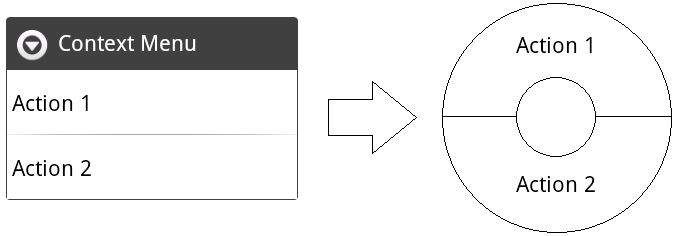
\includegraphics[scale = 0.5]{figure1.png} %
		\caption{Context menu and Marking menu}
		\label{linear-marking_menus}
\end{figure}

When a slice is selected or "marked", the sub-menu pops up and this, indefinitely until the user reaches an leaf item. We have a continual visual feedback of item browsing. The first mode corresponds to the novice mode. In the end, by repetitively using the novice mode, the user would memorize the gesture shape and would be able to draw directly it without even feeling the need of popping up the menu.

Hand-shape interfaces allow a very efficient interaction mode. For the purpose of enhancing the human interface, marking menus have been created but, to date, no android version exists.

\subsection{Usability}
This kind of menu is faster than a plain linear menu. It has been demonstrated that it is 3 times faster when the learning process is over. The muscle memory being a form of procedural memory, the body will remember gestures through repetition. The selecting action is then no longer a cognitive one.
To enhance the user experience marking menus follow the Fitts's law. If the distance and the size of an item are optimal, the time to reach it will be small. We are therefore working on a widget holding a great potential in terms of learning speed and efficiency.

\section{User experience}
We let dynamically and discretely the user choose between two modes. The choice will be realized depending on the amount of time the user presses the screen without moving. In order to completely understand the two modes developed in our project, we will see in the following parts screenshots of the menus/sub-menus browsing along with some explanations.

\subsection{Novice Mode}
For this mode, the user is discovering the menu and doesn't know any pattern. The menu is popping up every time. The central area is deprived of any component, corresponding to the size of a finger. Our marking menu is depicted in the following figure.

\begin{figure}[!ht] 
		\centering
		%\includegraphics[width=\columnwidth]{NS.png}
		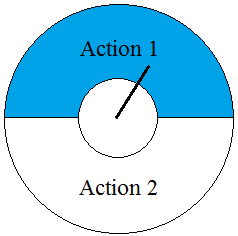
\includegraphics[scale = 0.5]{figure2.png} %
		\caption{Novice mode - action 1 marked}
		\label{linear-marking_menus}
\end{figure}

\subsection{Expert Mode}
After a learning process, the user masters the novice mode and becomes an expert. He can now easily navigate in the menu by drawing the pattern leading to the item he needs to reach without displaying the menu. If the pattern doesn't lead to a leaf item, a message is displayed on the screen indicating that the user has to try again.

\begin{figure}[!ht] 
		\centering
		%\includegraphics[width=\columnwidth]{NS.png}
		
\includegraphics[scale = 0.5]{figure3.png} %
		\caption{Expert mode - pattern recognition}
		\label{linear-marking_menus}
\end{figure}

\section{Constraints and assumptions}
Working in the mobile environment means you have to accept its constrains. The screen's size limits the user's motions. In the case of the marking menus it would at first makes us consider restricting the item number. Thus, we have decided to set up the number of items to 6. Beyond this value, it would be difficult to display the menu in novice mode and decrypt the scheme in expert mode. Plus, as long as we can make the menu pop up wherever we want, it would be a problem if we proceed actions at the edge of the screen. This have made us think about limiting as well the menu depth. 

\section{Effective implementation}
In order to provide something that could be integrated in the Android environment, we need to develop a widget in accordance with the standard official Android GUI procedure \cite{android}. Doing this make us first think about the visual representation of our menu and the way we will draw it. It turns out that a simple arc would fit the purpose \cite{touchmenotapps}. The distance to the finger where it will be drawn is deducted from the pythagorean theorem.

\begin{figure}[!ht] 
		\centering
		%\includegraphics[width=\columnwidth]{NS.png}
		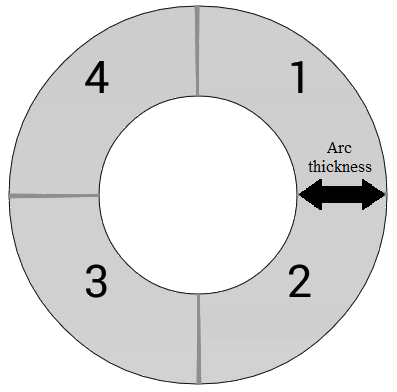
\includegraphics[scale = 0.5]{figure4.png} %
		\caption{Drawing the widget}
		\label{linear-marking_menus}
\end{figure}

When popping up the menu in novice mode at the edge of the screen, we apply an offset so that the depth limitation is no longer a problem. Plus our widget is not drawn truncated.

\begin{figure}[!ht] 
		\centering
		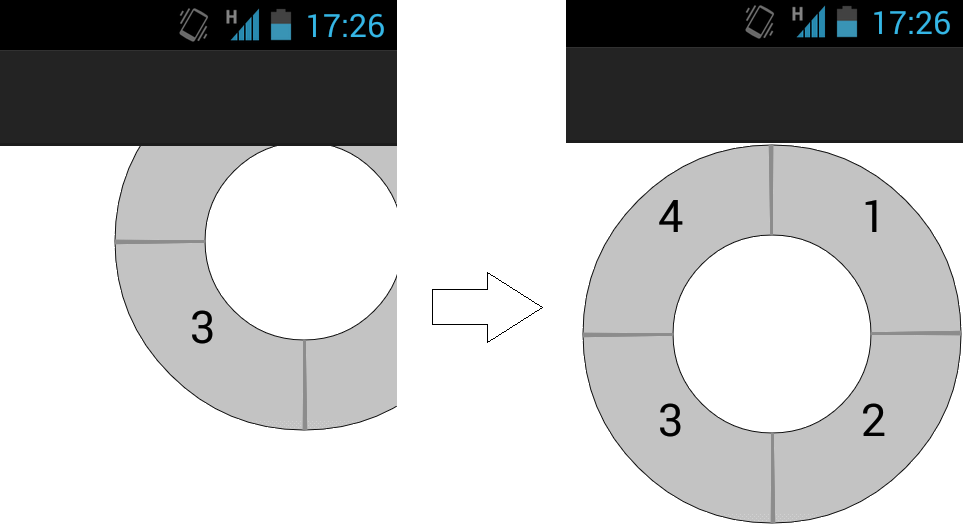
\includegraphics[width=\columnwidth]{figure5.png}
		%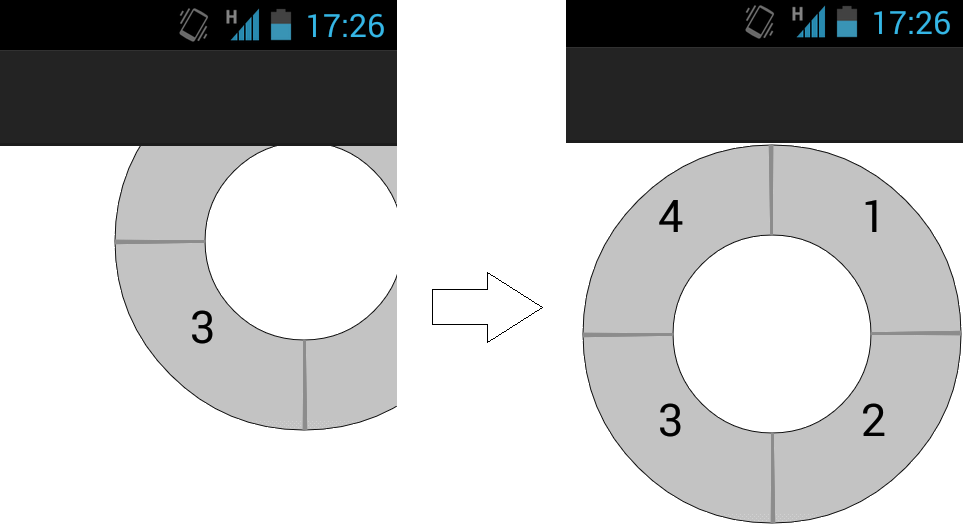
\includegraphics[scale = 0.5]{figure5.png} %
		\caption{Drawing at the edge of the screen}
		\label{linear-marking_menus}
\end{figure}

Regarding the expert mode, the main challenge in the scheme analysis is to determine how many inflection points there are. Because we have limited the number of items per level to 6, an inflection point should present an angle of at least 60\char23. In this way we are sure that a choice has been made by the user. But what if the choice was to go twice in the same direction? What are we supposed to do? We have chosen to display the menu from the novice mode to help the user know where he is and where he can go.

\begin{figure}[!ht] 
		\centering
		%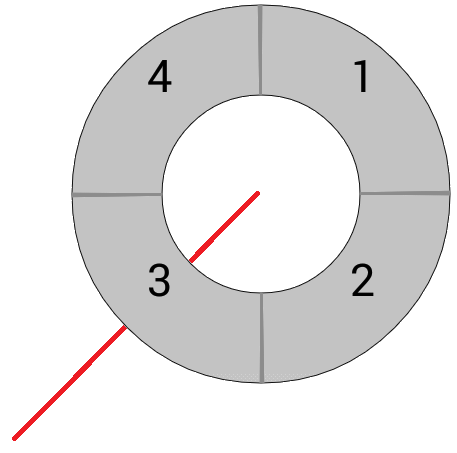
\includegraphics[width=\columnwidth]{figure6.png}
		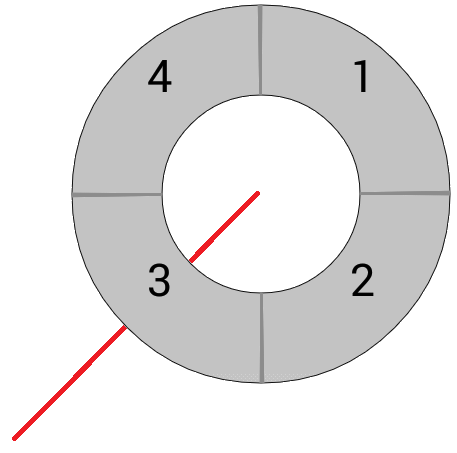
\includegraphics[scale = 0.5]{figure6.png} %
		\caption{Trying to go twice in the same direction}
		\label{linear-marking_menus}
\end{figure}

As long as we would like to let the users choose their menu structure, we provide a simple way of doing it. By means of an item object containing other item objects, we create a bedrock for user's customization.\\

\begin{thebibliography}{}
\bibitem{markingmenu}
http://www.markingmenus.org/
\bibitem{android}
http://developer.android.com/guide/topics/ui/custom-components.html
\bibitem{touchmenotapps}
https://github.com/strider2023/Radial-Menu-Widget-Android
\bibliographystyle{abbrv}
\end{thebibliography}

\end{document}
